\section{Operações com Conjuntos}
%\linespacedtitle

\subsection{Definições de Operações Básicas}
%\linespaced
As operações básicas com conjuntos constituem-se da reunião (ou união), interseção, diferença, complementar de um conjunto e diferença simétrica. Nas seções seguintes definimos tais operações e suas respectivas propriedades.

\subsubsection{Reunião de Conjuntos}

\begin{definition}
	Reunião de conjuntos. Chama-se a reunião (ou união) de conjuntos $A$ e $B$, o conjunto formado pelos elementos que pertencem a $A$ ou a $B$. 
	
	$$ A \cup B \; = \; \{ x | x \in A \; ou \; x \in B \} $$
	
\end{definition} 
%\linespaced

\noindent
\textbf{Propriedades da Reunião} 
%\linespacedtitle

\emph{A1. $ A \cup A \; = \;  A $ \; (Idempotente) }
\begin{proof}
	$ A \cup A \; = \; \{ x | x \in A \; ou \; x \in A \} \; = \; \{ x | x \in A\}$
\end{proof}


\emph{A2. $ A \cup \emptyset \; = \; A$ \; (Elemento Neutro) }
\begin{proof}
	$ A \cup \emptyset \; = \; \{ x | x \in A \; ou \; x \in \emptyset \} \; = \; \{ x| x \in A \}$
\end{proof}


\emph{A3. $ A \cup B \; = \; B\cup A $ \; (Comutativa)}
\begin{proof}
	$ A \cup B \; = \; \{ x | x \in A \; ou \; x \in B \} \; = \; \{ x | x \in B \; ou \; x \in A \}$
\end{proof}


\emph{A4. $( A \cup B ) \cup C \; = \; A \cup (B \cup C) $ \; (Associativa)}
\begin{proof} 
	
	$ A \cup B \; = \; \{ x | x \in A \; ou \; x \in B \} $ \\
	$ (A \cup B) \cup C \; = \; \{ x | (x \in A \; ou \; x \in B)  \; ou \; x \in C \} $ \\
	$ B \cup C \; = \; \{ x | x \in B \; ou \; x \in C  \} $ \\
	$ A \cup (B \cup C) \; = \; \{ x | x \in A \; ou \; (x \in B \; ou \; x \in C) \} \; = \;$ \\
	$\; = \; \{ x | x \in A \; ou \; x \in B \; ou \; x \in C \} \; = \; ( A \cup B) \cup C$
	
\end{proof}

\subsubsection{Interseção de Conjuntos}

Na interseção de conjuntos consideramos os elementos comuns à ambos os conjuntos. \\


\noindent
\textbf{Definição} Para conjuntos $A$ e $B$, a interseção de $A$ com $B$ é dada como, 

$$ A \cap B \; = \; \{x | x\in A \; e \; x \in B \} $$ 

Chama-se interseção de $A$ e $B$ o conjunto formado pelos elementos que pertencem à $B$ e à $A$. \\
%\linespacedEndSection


% Propriedades da interseção
\noindent
\textbf{Propriedades}
%\linespaced

\noindent
\emph{A1. $ A \cap A\; = \; A $ (idempotente)}

\noindent
\emph{A2. $A \cap U \;= \; A $ (elemento neutro) } 

\noindent
\emph{A3.  $ A \cap B \; = \; B \cap A $ (comutativa)}

\noindent
\emph{A4. $ A \cap ( B\cap C) \; = \; ( A \cap B ) \cap C $ (associativa)}


\subsubsection{Conjuntos Disjuntos}

Consideremos agora dois conjuntos $A$ e $B$ para os quais não há elemento em comum. Assim dizemos $A$ e $B$ são \textit{conjuntos disjuntos} definido como se segue.
%\linespaced
% Definição conjuntos disjuntos
\begin{definition}
	Conjuntos disjuntos são os conjuntos que não possuem elemento em comum, representado por $ A \cap B = \emptyset $.
\end{definition}

%\linespacedEndSection % espaçamento vertical em branco definido no preamble em 'main.tex'
\subsubsection{Propriedades da União e Interseção de Conjuntos} 

A seguir vejamos algumas propriedades envolvendo operações da união e interseção de conjuntos. Para tanto considere os conjuntos quaisquer $A$, $B$ e $C$. \\

\noindent
\textbf{Propriedades} \\
%\linespaced

\noindent
\emph{A1. $ A \cup (A \cap B) \; = \; A $ }
\begin{proof}
	$ A \cap B \; = \; \{ x | x \in A \; e \; x \in B \} $ 
	
	$ A \cup (A \cap B) \; = \; \{ x | x \in A \; ou \; (x \in A \; e \; x \in B) \}$
	
	$\; = \; \{ x | (x \in A \; ou \; x \in A) \} $
	
	$ = \; A $
	
\end{proof}

\noindent
\emph{A2. $ A \cap (A \cup B) \; = \; A$}
\begin{proof}
	$ A \cap (A \cup B) \; = \; \{ x | x \in A \; e \; (x \in A \; ou \; x \in B) \} $
	
	$ = \; \{ x | (x \in A \; e \; x \in A) \; ou \; (x \in A \; e \; x \in B) \} $ 
	
	$  = \{ x | x \in A \} \cup \{ x | x \in A \; e \; x \in B \} $ 
	
	$\; = \; A $
\end{proof} 

\noindent
\emph{A3. $A \cup (B \cap C ) \; = \; (A \cup B) \cap (A \cup C) $ }
\begin{proof}
	$ A \cup (B \cap C) \; = \; \{ x | x \in A \; ou \; (x \in B \; e \; x \in C)  \} \; = \; $
	
	$ = \; \{ x | (x \in A \; ou \; x \in B) \; e \; (x \in A \; ou \; x \in C) \} $
	
	$ = \; \{ x| x \in A \; ou \; x \in B \} \cap \{ x | x \in A \; ou \; x \in C \} $ 
	
	$ = \; (A \cup B) \cap (A \cup C) $  
	
\end{proof}

\noindent
\emph{A4. $  A \cap (B \cup C) \; = \; (A \cap B) \cup (A \cap C) $}
\begin{proof}
	$ A \cap ( B \cup C) \; = \; \{ x | x \in A \; e \; ( x \in B \; ou \; x \in C)  \} $
	
	$ = \; \{ x | (x \in A \; e \; x \in B) \; ou \; ( x \in A \; e \; x \in C)  \} $ 
	
	$ = \; \{ x | x \in A \; e \; x \in B \} \cup \{x | x \in A \; e \; x \in C \} $
	
	$ = \; (A \cap B) \cup (A \cap C)$
\end{proof}
%\linespacedEndSection


\subsubsection{Diferença de Conjuntos}

%\linespacedtitle

Dados conjuntos $A$ e $B$, definimos a diferença entre $A$ e $B$ como: 

	$$ A - B \; = \; \{ x | x \in A \; e \; x \notin B  \} $$.
	
Onde $A - B$ é o conjunto formado pelos elementos de $A$ que não pertencem a $B$. Chama-se o \textit{complementar de $B$ em relação a $A$} o conjunto $A - B$, representado por $C_A^B \; = \; A - B \; = \; C_A(B) = \bar{A}, \; (B \subset A) $. \\

%\linespaced
\noindent
\text{\maltese } Dados conjuntos $A$ e $X$ com $ X \subset A  $, o complementar dum conjunto  $X$, poderá ser escrito como, 

$$ C_A^X = A - X = C_A(X) $$

onde $C_A(X) = A - X  \; = \; \{\alpha \in C_A(X)| \ \alpha \in A \; e \; \alpha \notin X \} $. \\
%\linespaced

\text{\maltese} Consideraremos $C_U^A$ como $C(A)$ sendo o complementar de $A$ em relação ao conjunto universo U, onde $A \subset U$. \\

\noindent
\textbf{\underline{Exemplo}:}
	$ A \; = \; \{ a,b,c,d,e \}$, $B \; = \; \{ c,d,e \}$, $C_A^B \; = \; \{ a, b \}$ $(B \subset A)$. \\
	%\linespacedEndSection
	
	\noindent
	\textbf{Propriedades}
	%\linespaced
	\\
	
	\emph{A1. $ C_A^B \cap B = \emptyset $}
	\begin{proof}
		$ C_A^B \cap B \; = \; \{ x | (x \in A \; e \; x \in B) \} \cap \{ x | x \in B \} $\\

 		$ = \; \{ x | (x \in A \; e \; x \notin B) \; e \; x \notin B \} $\\

		$ =\; \{ x \in A | \underbrace{ x \in B \; e \; x \notin B}_{  = \; \emptyset } \} $\\ 

		$ = \; \{x \in A  \} \; = \; A, \; \text{pois } B \subset A $ \\

		$ x  \in C_A^B \Leftrightarrow x \notin B $ e o único conjunto \\

		$ \{ x \in A | x \in B \; e \; x \notin B \} \; = \; \emptyset $
	\end{proof}
	%\vspace{2mm}
	
	\emph{A2. $ C_ A^B \cup B\; = \; A$}
	\begin{proof}
		$ C_A^B \cup B \; = \; \{ x \in A | x \notin B \} \cup \{ x \notin B \} $ \\
		
		$ = \; \{ x \in A | x \notin B \; ou \; x \in B \} \; = \; A, $ pois $ B \subset A $ \\
	
		se $ x \in C_ A^B \Leftrightarrow x \notin B $. 
		
	\end{proof}
	%\vspace{2mm}
	
	\emph{A3. $C_A^A \; = \; \emptyset$} 
	\begin{proof}
		Se $x \in C_A^A \Leftrightarrow x \notin A$, o único conjunto $ \{ x| x \in A \; e \; x \notin A  \} $ é o vazio. 
	\end{proof}
	%\vspace{2mm}
	
	\emph{A4. $ C_A^{\emptyset} = A $}
	\begin{proof}
		Se $ x \in C_ A^\emptyset \Leftrightarrow x \notin \emptyset \; = \; A $
	\end{proof}
	%\vspace{2mm}
	
	
	\emph{A5. $ C_A^{(B \cap C)} \; = \; C_ A^B \cup C_A^C $}
	%\linespaced
	
	\begin{proof}
		Se $x \in C_A^{(B \cap C )} \Leftrightarrow x \notin B \cap C $\\
		
		$= \; \{ x \in A | x \notin B \cap C \} \; = \; \{ x \in A | x \notin B \; ou \; x \notin C  \} $ \\
		
		$ = \; \{ x \in A | x \notin B \} \cup \{ x \in A | x \notin C \} $ \\
		
		$ = \;C_A^B \cup C_A^C $ \\		
		
	\end{proof}
	%\vspace{2mm}
	
	\emph{A6. $ C_ A^{(B \cup C)} \; = \; C_A^B \cap C_A^C $ }
	%\linespaced
	\begin{proof}
		$ C_A^{(B \cup C)} \; = \; \{ x \in A | x \notin (B \cup C)  \} $ \\
		
		$ = \; \{ x \in A | x \notin B \; e \; x \notin C \} $ \\
		
		$ = \; \{ x \in A | x \notin B \} \cap \{ x \in A | x \notin C \} $ \\
		
		$ = \; C_A^B \cap C_A^C $
		
	\end{proof}
	%\vspace{2mm}
	
	\emph{A7. $ C_A^{(C_A^B)} \; = \; B $}
	\begin{proof}
		$ C_ A^{C_A^B}  \; = \; \{ x \in A | x \notin C_A^B  \}$ \\
		
		$ = \; \{ x \in A | x \notin (x \in A | x \notin B)  \} $ \\
		
		$ = \; \{ x \in A | x \in B \} \; = \; B \subset A $ \\
		
		como $ B \subset A \Rightarrow \{ x \in B \Rightarrow x \in A \}$, $ \forall x$. \\
		 
		$ \bar{A} \; = \;A - B$, ou $ x \in B$ ou $x \in \bar{A} $ \\
		
		se $ x \in C_A^{C_ A^{B}} \Leftrightarrow x \notin C_ A^B \Leftrightarrow x \in B $ e como $B \subset A$ \\
		
		$ \Rightarrow C_ A^{C_A^B} \; = \; B $
		
	\end{proof}
	%\vspace{2mm}

	\pagebreak

\subsubsection{Diferença Simétrica} 
%\linespaced
\noindent
Dados os conjunto $A$ e $B$,
$$ A \Delta B = ( A - B ) \cup ( B - A ) $$
é a diferença simétrica dos conjuntos $A$ e $B$. \\
%\linespaced

\noindent
\underline{Exemplo}: $ A = \{ a, b, c, d \}$ e $ B = \{ c, d, e, f, g \} $ \\ \\
$$ A - B = \{ a, b, c, d \} - \{ c, d, e, f, g \} = \{ a, b \} $$ \\
$$ B - A = \{ c, d, e, f, g \} - \{ a, b, c, d \} = \{ e, f, g \}  $$ \\
$$ ( A - B ) \cup ( B - A ) = \{ a, b \} \cup \{ e, f, g \} = \{ a, b, e, f, g  \}$$ \\
%\linespaced

% Continuar da página 19 (diferença simétrica, propriedades)
\noindent
\underline{Propriedades} \\

\noindent
\emph{i)} $ A \Delta A = \emptyset$ \\
\noindent
\begin{proof}
	$ A \Delta A = (A -A ) \cup (A - A) = \emptyset \cup \emptyset = \emptyset $ \\
\end{proof}

\noindent
\emph{ii)} $ A \Delta \emptyset = A $ \\
\noindent
\begin{proof}
	$ A \Delta \emptyset = ( A - \emptyset) \cup (\emptyset - A ) = A \cup \emptyset = A $ \\
\end{proof}

\noindent
\emph{iii)} $ A \Delta B = B \Delta A $ \\
\noindent
\begin{proof}
	$ A \Delta B = (A - B ) \cup ( B - A ) = ( B - A ) \cup ( A - B )= B \Delta A $
\end{proof}
%\linespaced %\linespaced
% Gráficos
% \tikz \fill[even odd rule] (0,0) circle (1) (1,0) circle (1);

\begin{center}

%Fig. 1
\begin{tikzpicture}
\centering
% Set A
\draw [pattern=north east lines] (0, 0) circle (1.2cm);
\draw (-1.4, 0.5 ) node {$A$};
\draw [->] (-0.8, 0.2) -- (-2, -0.6);
\draw (-2.3, -0.9) node {$A - B$};
% Set B	
%\filldraw [fill=white, draw=black] (1,0) circle (0.8cm);
\draw [pattern=north east lines] ( 1.2, 0) circle (1.2cm);
\draw (2.5, 0.5) node {$B$};
\draw [->] (2.0, 0.2) -- (2.6, -0.6);
\draw (2.9, -0.9) node {$ B - A $};

% Intersection
\begin{scope}
\clip (0,0) circle(1.2cm);
\clip (1.2,0) circle(1.2cm);
\filldraw [fill=white] (0.5, 0) circle (1.2cm) node {$A \cap B $};
\end{scope}

%\filldraw [fill=white, draw=black] (0, 0 ) circle (0.4cm) node [fill=white] {$B$}; 
\draw (0, -2.0 )node {\text{Fig.1: Há interseção entre $A$ e $B$} };
\end{tikzpicture}
% Fig. 2
\begin{tikzpicture}
% Set A
\draw [pattern=north east lines] (0, 0) circle (1.2 cm);
\draw (-1.5, 0.5) node {$A$};
% Set B
\filldraw [fill=white, draw=black] (0.3, -0.5) circle (0.5cm) node [fill=white] {$B$};
\draw (0, -2.0 )node {\text{Fig.2: } $ B \subset A$};
\draw [->] (0.6, 0.6) -- (1.8, -0.4);
\draw (2.0, -0.8) node {$ A - B = C_A^B $};
\end{tikzpicture}
%\linespaced
% Fig. 3
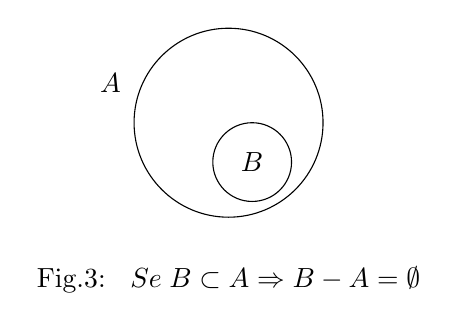
\begin{tikzpicture}
% Set A
\draw [] (0, 0) circle (1.2 cm);
\draw (-1.5, 0.5) node {$A$};
% Set B
\filldraw [fill=white, draw=black] (0.3, -0.5) circle (0.5cm) node [fill=white] {$B$};

\draw (0, -2.0 )node {\text{Fig.3: } $ Se \; B \subset A \Rightarrow B - A = \emptyset$};
\end{tikzpicture}
%\linespaced %\linespaced %\linespaced
\end{center}

\noindent
Considerando diagramas anteriores (Figs 1, 2 e 3), \\ \\
$ A \Delta B = ( A - B)  \cup (B - A)$ \\

\noindent
se $ B \subset A \Rightarrow B - A = \emptyset $ e $ A - B = \{x | x \in A \ e \ x \notin B\} \qquad \text{(Fig 3)}$ \\

\noindent
$ \Rightarrow A \Delta B = ( A - B ) \cup \emptyset = C_A^B \cup \emptyset = C_A^B$ \\ \\

%\linespaced
\noindent
\text{\maltese} $A \cap B = \{ x | x \in A \; e \; x \in B \} $ \\
$ A - B = \{ x \in A | x \notin B \} $ \\
$ ( A \cap B ) \cup ( A - B ) = \{ x |  x \in  A \ e \ x \in B \} \cup \{ x \in A | A  x \notin B \} $ \\
$ = \{ x | \; (x \in A \; e \; x \in B) \; ou \; ( x \in A \; e \; x \notin B ) \} = $ \\
$ = x \in (A \cap B) \cup(A - B) \Rightarrow x \in (A \cap B) \; ou \; x \in (A - B) \\ \Leftrightarrow ( x \in A \; e \; x \in B) \; ou \; ( x \in A \; e \; x \notin B ) $ \\
$ \Leftrightarrow \{ x \in A | x \in A \; e \; x \in B \} = A \cap B$ \\

\subsection{Exercícios Resolvidos}

% Exercícios
%\emph{\textbf{\underline{Exercícios Resolvidos}}}
%\linespacedtitle
	
Considerando os conjuntos $A$, $B$ e $D$, onde 
$A \; = \; \{ a, b, c, d \}$, $ B \; = \; \{ c, d, e, f, g \} $ e $ D \; = \; \{ b, d, e, g \} $. (1-6)  
	 
\begin{enumerate}
% 1º
\item 
$ A - B \; = \; \{ a,b \}$ \\
			
% 2º
\item 
$ B - A \; = \; \{ e, f, g \} $ \\
		
%3º
\item 
$ D - B \; = \; \{ b \} $ \\
		
%4º
\item 
$ (A \cup D) - B\; = \; \{  a, b \}  $ \\
		
% 5º
\item 
$ A - (B \cap D) \; = \;\{ a, b, c \} $ \\
		
% 6º
\item 
$  (A \cup B) - ( A \cap D) \; = \; \{ a, b, c, d, e, f, g \} - \{ b, d \} \; $
$ = \; \{ a, c, e, f, g \} $ \\
		
% 7º
\item 
$ A \; = \; \{ a, b, c, d, e, f \}$, $ B \; = \; \{ b, c, d \} $ \\ \\

$ A - B \; = \; \{ a, e, f \} \; = \; C_A^B $, pois $ B \subset A $. \\ \\

$ C_A^B \cap B \; = \; \{ a, e, f \} \cap \{b, c, d\} \; = \; \emptyset $ \\ \\

$ C_A^B \cup B \; = \; \{ a, e, f \} \cup \{ b, c, d \} \; = \; \{ a, b, c, d, e, f \} \; = \; A $ \\ \\

$ C_A^{(C_ A^B)} \; = \; C_A^{\{ a, e, f \}} \; = \; \{ b, c, d \} \; = \; B $  \\ \\

se $ D = \{e, f\} \Rightarrow C_A^D \; = \; \{ a, b, c, d \}  $ \\ \\

$ C_A^B \cup C_A^D \; = \; \{ a, e, f \} \cup \{ a, b, c, d \} \; = \; \{ a, b, c, d, e, f \} $ \\ \\

$ B \cap D \; = \; \{ b, c, d \} \cap \{ e, f \}  \; = \; \emptyset $ \\ \\

\text{\maltese} Se $ A \; = \; B \cup C \Rightarrow 
\begin{cases}
C_A^B \cup C_A^C = C_A^{\emptyset} = A \\
C_A^B \cap C_A^C = C_A^A = \emptyset
\end{cases} $\\

\begin{center}
% Diagrama para o conjunto dado por A - B
\begin{tikzpicture}

\draw [pattern=north east lines ] (0, 0) circle (0.9cm) ;
\draw (-0.3, -1.15) node {$A$};
\draw [->] (0.4,0.4)  -- (0.5,1.1);
\draw (0.7,1.3) node   {$ A - B \; = \; \bar{B} \; = \; C_A^B$};
\filldraw [fill=white, draw=black] (0, 0 ) circle (0.4cm) node [fill=white] {$B$}; 

\end{tikzpicture}
\end{center}

Por definição se $x \in C_A^B \Leftrightarrow x \notin B$. \\ \\

\text{$(\ast)$ } $ A - \bar{B} = A \cap B$, onde $ A \subset U $ e $ B \subset U $, $A$ e $B$ são quaisquer. \\

\underline{Prova} \\
Se $x \in (A - \bar{B}) \Rightarrow x \in A $ e $x \notin \bar{B} \Rightarrow x \in A$ e $x \in B \Rightarrow x \in A \cap B$, $ \forall x$. 	

		
\end{enumerate}

	

\newpage


\subsection{Exemplos}

%\linespacedtitle
\textbf{\underline{Exemplo 1}} $ A \cup (B \cap C) =  (A \cup B) \cap (A \cup C) $  \\ \\
%\linespaced
\underline{Prova:} \text{$ \Rightarrow $}  Se $ x \in A \cup (B \cap C) \Rightarrow x \in A \; ou \; x \in (B \cap C) $ \\
%\linespaced
(i) $ x \in A \; ou \; x \in B \Rightarrow x \in A \cup B $ \\
(ii) $ x \in A \; ou \; x \in C \Rightarrow x \in A \cup C $ \\

$ \Rightarrow  x \in A \cup B$ e $ x \in A \cup C \Rightarrow x \in (A \cup B) \cap (A \cup C)$ \\

$ \Leftarrow  $ Se $ x \in (A \cup B) \cap(A \cup C) \Rightarrow x \in (A \cup B) \; e \; x \in (A \cup C) $ \\

$ \Rightarrow$ ou $x \in A \text{ ou } x \in A \cup (B \cap C) $ \\

$x \notin A \Rightarrow x \in B \; e \; x \in C \Rightarrow x \in B \cap C $ \\

$ \Rightarrow x \in A \cup (B \cap C) $  

\begin{flushright}
	\textit{C.Q.D} \\
\end{flushright}

\noindent
\textbf{\underline{Exemplo 2}} Se $ A \cap B \neq \emptyset$, ou seja, existe o conjunto não vazio \\  $\{ x | x \in A \; e \; x \in B \} $. \\



\begin{wrapfigure}{l}{0.35\textwidth}
	\centering
	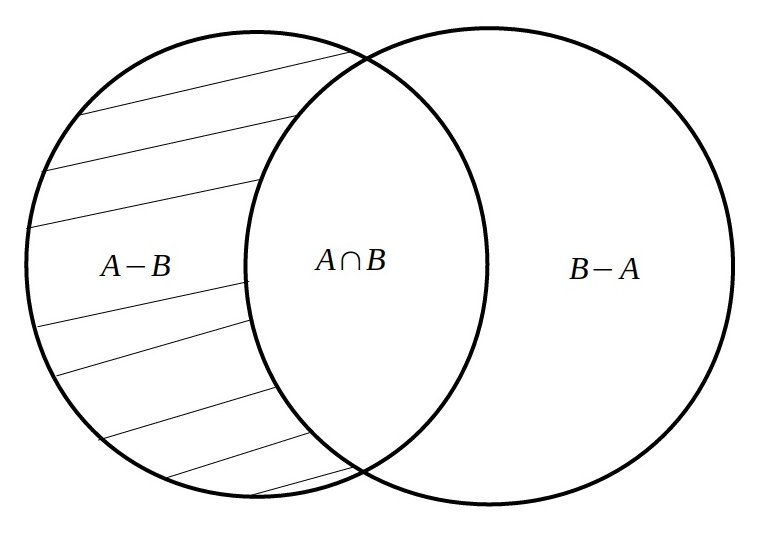
\includegraphics[width=0.35\textwidth]{math1}
\end{wrapfigure}

\noindent
$ A - B  = \{ x | x \in A \; e \; x \notin B\}$ 
%\linespaced

\noindent
Não se exige que $ B \subset A $ para que exista $ A - B $, de fato podemos escrever $ A - B \;= \; A - (A \cap B) $, sendo essa operação válida para quaisquer $A$ e $B$. \\ \\ \\
\linebreak

\noindent
Quando $\emptyset \; = \; A \cap B \Rightarrow A - B = C_A(B) $.  \\
Quando $ B \subset A \Rightarrow A - B = C_A(B) $, $ x \in C_A(B) \Leftrightarrow x \notin B$ \\
%\linespaced

\noindent
\textbf{\underline{Exemplo 3}} 
$ A = \{ x \in \mathbb{Z} | x \geq -3 \} $ e $ A = \{ x \in \mathbb{Z} | x \leq 2 \}$, 

%\linespaced
\noindent
$A - B \; = \; \{ x \in \mathbb{Z}| x \geq 3 \}$, $B - A =\{x \in \mathbb{Z} | x \leqslant -4 \} $ \\
$C_A^{\mathbb{Z}} = \{ \text{inteiros menores que -3}\} $
%\linespaced

\noindent
$ C_B^{\mathbb{Z}} = \{ \text{inteiros maiores que 2} \} $ 

%\linespaced

\noindent
\textbf{\underline{Exemplo 4}} Seja $E$ um conjunto fundamental e $ A \subset E $ e $ B \subset E $.
$$ A - B \; = \; A \cap C_B^E $$

\noindent
\underline{Prova:} $ x \in (a - B)  \Leftrightarrow x \in A \; e \; x \notin B \Leftrightarrow  x \in A \; e \; x \in C_B^E $ \\
$ \Leftrightarrow \{ x \in E | x \in A \} \cap \{ x \in E | x \notin B \} \Leftrightarrow A \cap C_B^E $ \\

%\linespaced
\noindent
\textbf{\underline{Exemplo 5}} $ C_A^{C_A^E} \; = \; E $ \\

\noindent
\underline{Prova: } $ x \in C_A^{C_A^E} \Leftrightarrow x \notin C_A^E \Leftrightarrow x \in A \Rightarrow C_A^{C_A^E} = A $ \\

\noindent
\textbf{\underline{Exemplo 6}}  $ A \subset B \Leftrightarrow C_B^E \subset C_A^E $ 
%\linespaced

\noindent
\underline{Prova:} $(\Rightarrow)$ $ A \subset B \Rightarrow (x \in A \Rightarrow x \in B) $ então $ x \in C_B^E $ não pode pertencer a $B$, mas isso implica por construção que $x \notin A$ ($ x \in C_B^E \Rightarrow x \in C_A^E$) ou seja $ C_B^E \subset C_A^E $. \\

\noindent
$( \Leftarrow )$ Supondo $ C_B^E \subset C_A^E \Rightarrow ( x \in C_B^E \Rightarrow x \in C_A^E) $  então \\ $ x \in C_A^{C_A^E} $ não pode pertencer a $ C_A^E $, isso implica que $x \notin C_B^E $ por construção $ ( x \in C_A^{C_A^E}) \Rightarrow x \in C_B^{C_B^E} \sim (x \in A \Rightarrow x \in B )$, ou seja $ A \subset B $. Onde usamos o resultado $ C_A^{C_A^E} = A $ e $ C_B^{C_B^E} = B $. \\
%\linespaced

\noindent
\text{\maltese } Se $ A = \emptyset \Leftrightarrow C_A^E = E $. \\

\noindent
\underline{Prova: } $ A = \emptyset \Leftrightarrow x \notin A, \; \forall x \in E \Leftrightarrow x \in C_A^E, \; \forall x \in E \Leftrightarrow C_A^E = E $. \\
%\vspace{18mm}
%\linespaced

\noindent
\text{\maltese } $ C(A \cup B) = C_A^E \cap C_B^E $ \\

\noindent
\underline{Prova}: $A \subset (A \cup B) \Leftrightarrow C_{A \cup B}^{E} \subset C_A^E$ e $ B \subset (A \cup B) \Leftrightarrow C_{A \cup B}^E \subset C_B^E \Rightarrow C_{A \cup B}^E \subset C_A^E \cap C_B^E $. \\

%\linespaced
\noindent
\text{\maltese } Seja $ X = C_A \cap C_B \Rightarrow X \subset C_A \; e \; X \subset C_B$ \\

$ \Rightarrow ( X \subset C_A \Leftrightarrow C_A(C_A) \subset C_X) \Leftrightarrow ( X \subset C_A \Leftrightarrow A \subset C_X ) $ \\

$ \Rightarrow ( X \subset C_B \Leftrightarrow C_B(C_B) \subset C_X ) \Leftrightarrow ( x \subset 
C_B \Leftrightarrow B \subset C_X ) $ \\

como $ ( A \subset C_X \; e \; B \subset C_X ) \Leftrightarrow ( A \cup B \subset C_X ) $ \\

$ \Leftrightarrow ( A \cup B \subset C_X  \Leftrightarrow  C_X(C_X) \subset C_{A \cup B})  \overset{\mathit{C_X(C_X) = X}} \Longleftrightarrow ( X \subset C_{A \cup B} )$ \\

$ \overset{X = C_A \cap C_B} \Longleftrightarrow ( X \subset C_{A \cup B} ) $ \\
\begin{flushright}
	\textit{C.Q.D} \\
\end{flushright}

%\linespaced
\text{\maltese } $ C(A \cap B) = C_A \cup C_B $\\

\underline{Prova:} Análogo a prova anterior. \\
\newpage

\noindent
\textbf{Diagramas}
\begin{center}  
% Reprensentação das operações dos conjuntos por diagramas de Venn

	\centering
	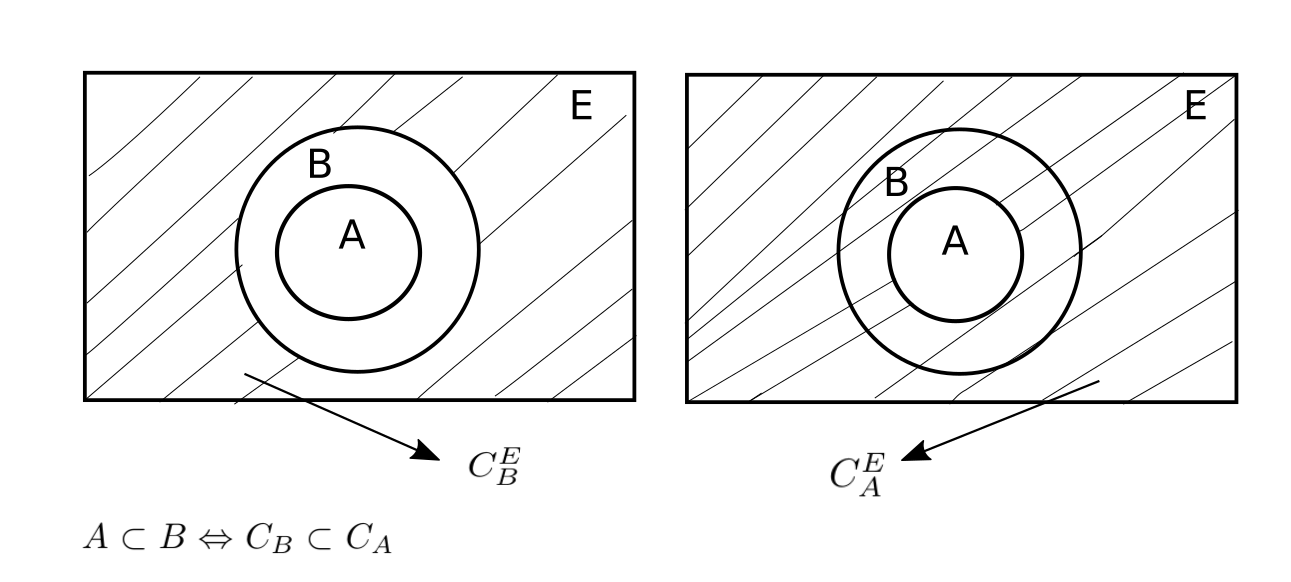
\includegraphics[scale=0.2]{conjuntos-sec2-1}



	\centering
	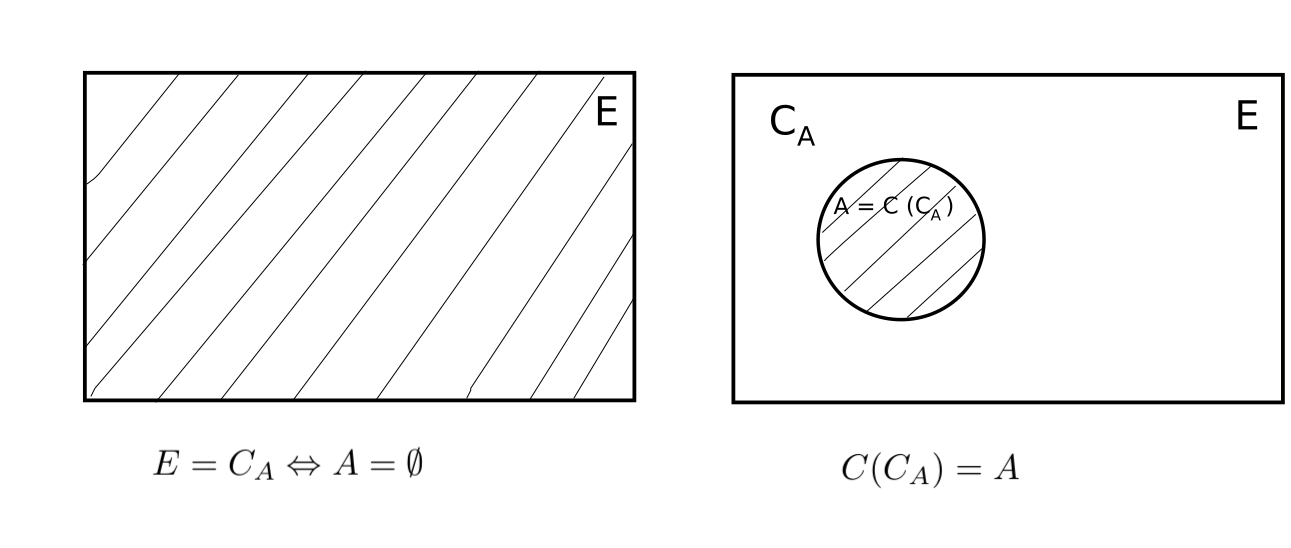
\includegraphics[scale=0.2]{conjuntos-sec2-2}
	


	\centering
	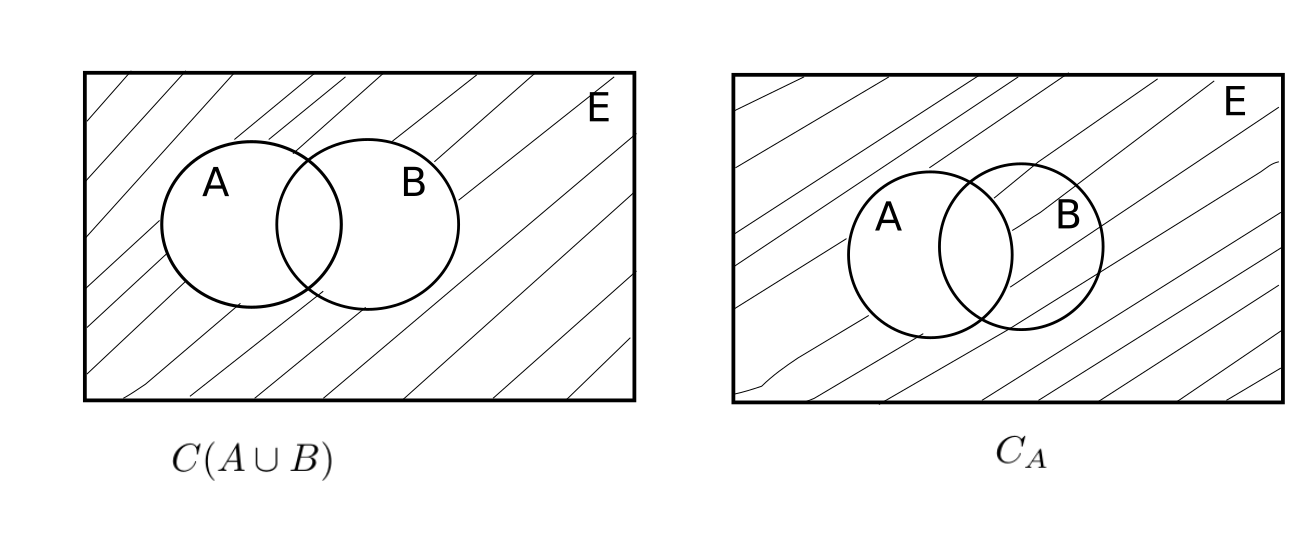
\includegraphics[scale=0.2]{conjuntos-sec2-3}



	\centering
	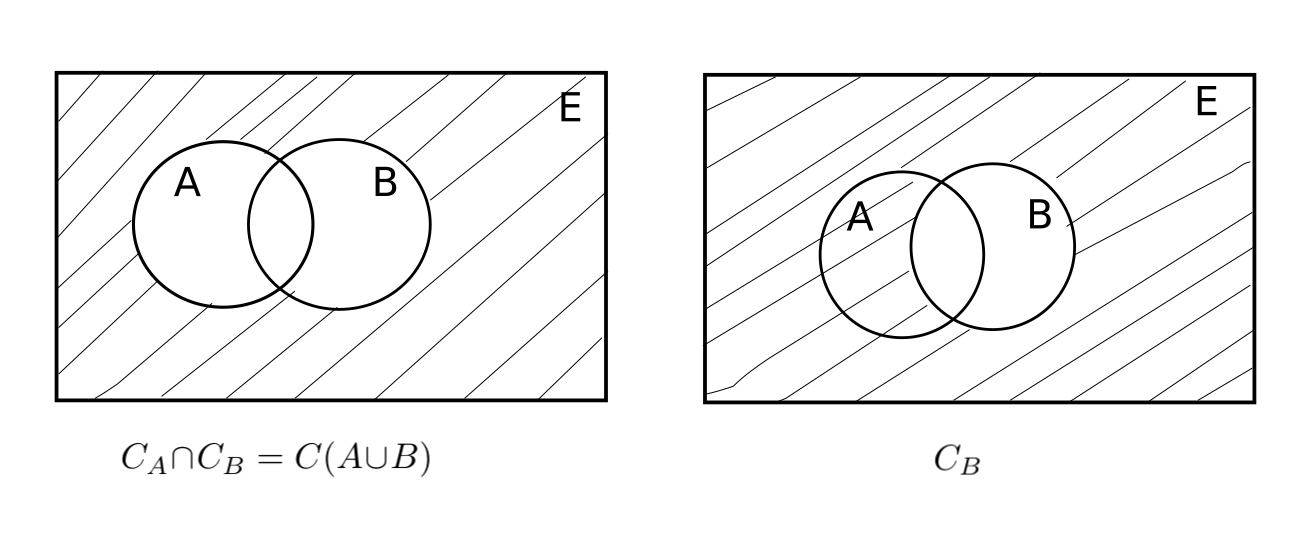
\includegraphics[scale=0.2]{conjuntos-sec2-4}



	\centering
	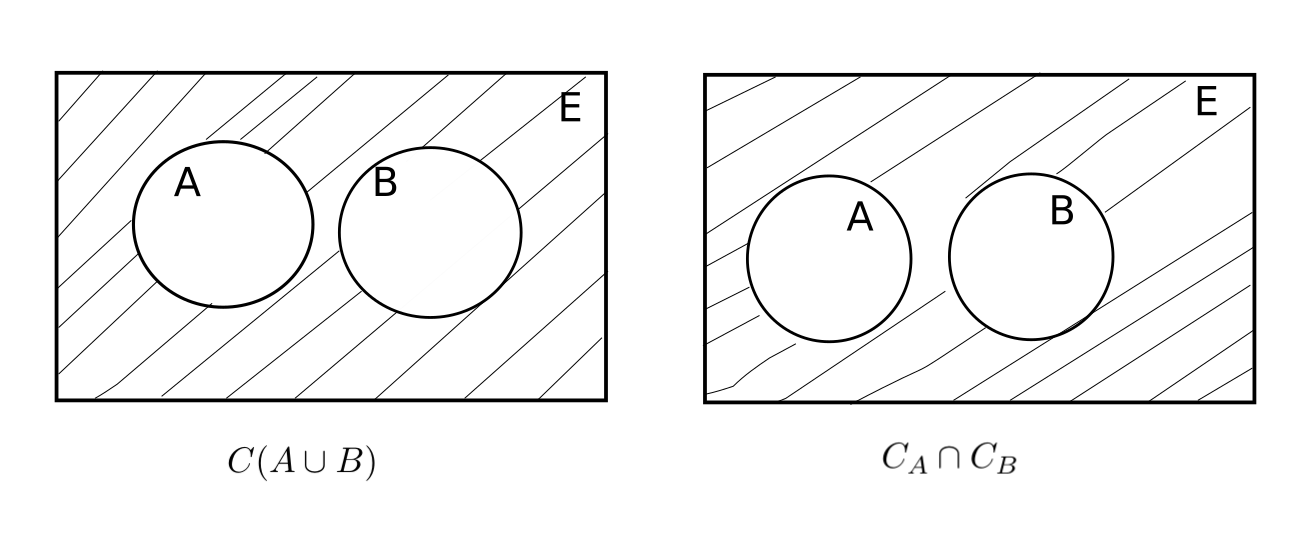
\includegraphics[scale=0.2]{conjuntos-sec2-5}



	\centering
	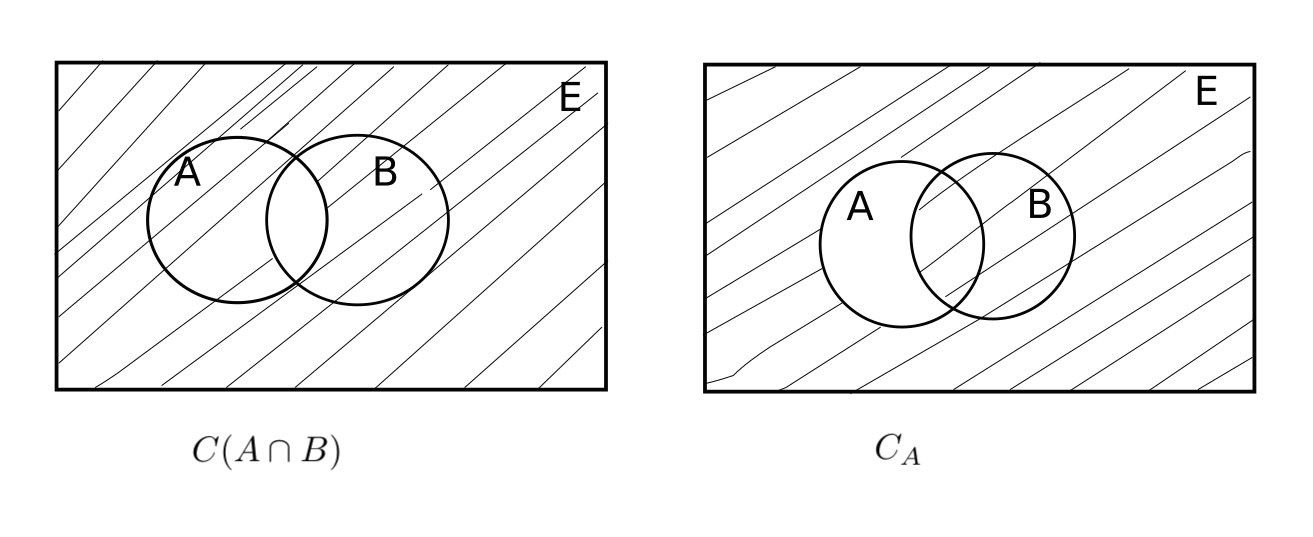
\includegraphics[scale=0.2]{conjuntos-sec2-6}



	\centering
	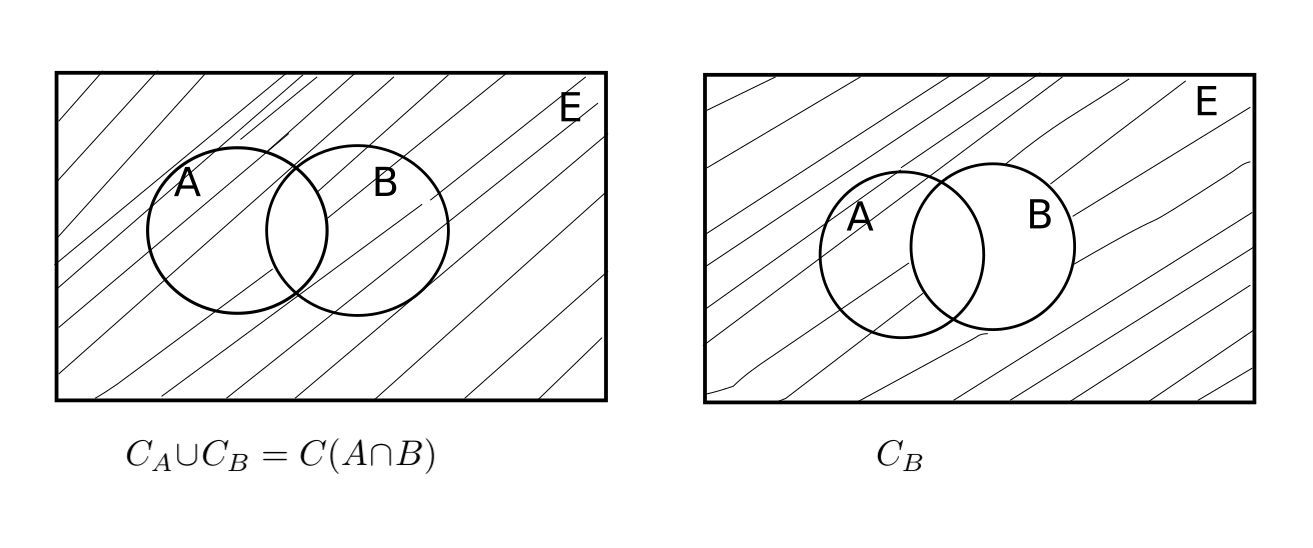
\includegraphics[scale=0.2]{conjuntos-sec2-7}

\end{center}

%\linespaced
\text{\maltese } Se $ ( X \supset A \; e \; X \supset B) , \; ( Y \supset A \; e \; Y \supset B)  \Rightarrow Y \supset X $  \\
$ \Rightarrow X = A \cup B  $.
\noindent
\begin{proof}
	%\linespaced
	$  \Rightarrow A \subset X \; e \; B \subset X \Rightarrow A \cup B \subset X $ \\
	se $ A \subset Y \; e \; B \subset Y \Rightarrow X \subset Y $ \\
	$ A \subset Y \; e \; B \subset Y \Rightarrow A \cup B \subset Y \Rightarrow X \subset Y $ \\ \\
	$
	\begin{cases}
		  (A \cup B ) \subset X \; e \; ( A \cup B ) \subset Y \Rightarrow X \subset Y \\
		  A \cup B \subset X \Rightarrow \{ x \in X | x \in A \cup B \} 
	\end{cases} $ \\ \\

	\noindent
	$ ( A \cup B ) \subset Y \Rightarrow X \subset Y \Leftrightarrow ( ( x \in A \cup B \Rightarrow  x \in Y )  \Rightarrow ( x \in X \Rightarrow x \in Y ) ) $ \\ \\
	$x \in A \cup B \Rightarrow  x \in X   \qquad\qquad	( Z = A \cup B \subset X ) $
	
	\noindent
	$ A \cup B \subset Y \Rightarrow ( x \in A \cup B = Z \Rightarrow x \in Y ) $ \\ \\
	\noindent
	$ \Rightarrow X \subset Y \Rightarrow ( x \in X \Rightarrow x \in Y )$ \\ \\
	$  ( x \in Z \Rightarrow x \in X \Rightarrow x \in Y ) $ \\ \\
	$ ( x \in Z \Rightarrow x \in Y ) \Rightarrow ( x \in X \Rightarrow x \in Y ) $ \\ \\
	
	\fbox{$ X \cap ( A \cup B ) = X = A \cup B $} \\ \\
	
	$\begin{cases}
		 A \cup B \subset X  \\
		( A \cup B \subset Y \Rightarrow X \subset Y ) \Rightarrow X \subset A \cup B \\ \\
	\end{cases}$\\ \\

	\noindent
	$ A \cup B \subset \ X e \ X \subset A \cup B \Rightarrow X = A \cup B $ 
	
\end{proof}

\noindent
\textbf{\underline{Exemplo}} \\

\noindent
\emph{(1)} $ (A \cup B ) \cap C \ne A \cup ( B \cap C ) $ \\ \\
Considere
$\begin{cases}
 A \cup ( B \cap C ) = ( A \cup B ) \cap ( A \cup C ) \\
 C \cap ( A \cup B ) = (C \cap A ) \cup ( C \cap B )
\end{cases}$  
%\linespaced

Tomemos os conjuntos $ A = \{ a,b,c \} $,  $ B = \{ e, f, g, h \} $ e $ C = \{ d, e \} $ como exemplos, \\ \\
$ ( A \cup B ) \cap C = \{ a, \ b, \ c, \ e, \ f, \ g, \ h \} \cap \{ d, \ e \} = \{ e \} $ \\ \\
porém, \\ \\
$ A \cup ( B \cap C ) = \{ a, b, c \} \cup \{ e \} = \{a, \ b, \ c, \ e \}$. \\

%\vspace{18mm}